Having introduced \pred, we now investigate its performance in diverse bandit settings compared to other in-context learning algorithms.
% 
In our first set of experiments, we use a bandit setting with a common non-linear structure across tasks.
% In this section, we study non-linear structured bandit setting. In a non-linear structured bandit regime, every task has a non-linear reward structure which is common to real-life datasets. 
Ideally, a good learner would leverage the structure, however, we choose the structure such that no existing algorithms are well-suited to the non-linear structure.
% 
This setting is thus a good testbed for establishing that in-context learning can discover and exploit common structure.
% Therefore any good learner must learn to leverage the structure across the tasks and predict the best outcome for new unseen tasks at test time. 
% In a non-linear structured bandit regime, every task has a non-linear reward structure. Therefore any good learner must learn to leverage the structure across the tasks. 
%
Moreover, each task only consists of a few rounds of interactions.
%
This setting is quite common in recommender settings where user interaction with the system lasts only for a few rounds and has an underlying non-linear structure \citep{kwon2022tractable, tomkins2020rapidly}.
%
We show that \pred\ achieves lower regret than other in-context algorithms for the non-linear structured bandit setting. 
%
% We also analyze the exploration strategy of \pred\ (\gt) in this setting.
%
We study the performance of \pred\ in the large horizon setting in \Cref{sec:horizon}. 


\textbf{Baselines:} We first discuss the baselines used in this setting.

\noindent
\textbf{(1) \pred:} This is our proposed method shown in \Cref{alg:pred}.

\textbf{(2) \predt:} This is the proposed exploratory method shown in \Cref{alg:pred} and we fix $\tau=0.05$. 

\textbf{(3) \dptg:} This baseline is the greedy approximation of the \dpt\ algorithm from \citet{lee2023supervised} which is discussed in \Cref{sec:prelim-dpt}.
%
Note that we choose \dptg\ as a representative example of similar in-context decision-making algorithms studied in \citet{lee2023supervised, sinii2023context, lin2023transformers, ma2023rethinking, liu2023reason, liu2023self} all of which require the optimal action (or its greedy approximation). 
%We choose \dpt\ as a representative example of this learning procedure.
%
\dptg\ estimates the optimal arm using the reward estimates for each arm during each task. %uses training data $\Htr$ to estimate the optimal action for each task $m$. 
%
% For each task $m$, \dptg\ evaluates the optimal action $\widehat{a}_{m,*} = \argmax_a \sum_{t=1}^n\wr_{m,t}(a)$ where, $\wr_{m,t}(a) = \sum_{t=1}^n \wr_{m,t}\mathbf{1}(I_t =a)$ is the observed cumulative reward for the action $a$ in task $m$ and $\mathbf{1}(\cdot)$ is the indicator function. Note that the optimal action $\widehat{a}_{m,*}$ is evaluated using the entire dataset $\H_m$. Finally, it implements the training procedure as discussed in \Cref{sec:prelim-dpt}. 
 
\textbf{(4) \ad:} This is the Algorithmic Distillation method \citep{laskin2022context, lu2021low} discussed in \Cref{sec:prelim-dpt}. 

\textbf{(5) \ts:} This baseline is the celebrated stochastic $A$-action bandit Thompson Sampling algorithm from \citet{thompson1933likelihood,agrawal2012analysis,russo2018tutorial,zhu2020thompson}.
%
We choose \ts\ as the weak demonstrator $\pi^w$ as it does not make use of arm features.
% 
\ts\ is also a stochastic algorithm that induces more exploration in the demonstrations. 

\textbf{(6) \linucb:} (Linear Upper Confidence Bound): This baseline is the Upper Confidence Bound algorithm for the linear bandit setting that leverages the linear structure and feature of the arms to select the most promising action as well as conducting exploration. We choose \linucb\ as a baseline for each test task to show the limitations of algorithms that use linear feedback structure as an underlying assumption to select actions. Note that \linucb\ requires oracle access to features to select actions per task.


\textbf{(7) \mlin:} This is the multi-task linear regression bandit algorithm proposed by \citet{yang2021impact}. This algorithm assumes that there is a common low-dimensional feature extractor shared between the tasks and the reward of each task linearly depends on this feature extractor. We choose \mlin\ as a baseline to show the limitations of algorithms that use linear feedback structure \textit{across tasks} as an underlying assumption to select actions. Note that \mlin\ requires oracle access to the action features to select actions as opposed to \dpt, \ad, and \pred.

We describe in detail the baselines \ts, \linucb, and \mlin\ for interested readers in \Cref{app:baseline-details}.

% \textbf{(5) \ts:} This baseline is the stochastic $A$-action bandit Thompson Sampling algorithm from \citet{thompson1933likelihood,agrawal2012analysis,russo2018tutorial,zhu2020thompson}. We briefly describe the algorithm below: At every round $t$ and each action $a$, \ts\  samples $\gamma_{m,t}(a) \sim \N(\wmu_{m,t-1}(a), \sigma^2/N_{m,t-1}(a))$, where $N_{m,t-1}(a)$ is the number of times the action $a$ has been selected till $t-1$, and $\wmu_{m,t-1}(a) = \frac{\sum_{s=1}^{t-1} \wr_{m,s}\mathbf{1}(I_s =a)}{N_{m,t-1}(a)}$ is the empirical mean. Then the action selected at round $t$ is $I_{t} = \argmax_a \gamma_{m,t}(a)$. 
% %
% Observe that \ts\ is not a deterministic algorithm like \ucb\ \citep{auer2002finite-time}. So we choose \ts\ as the weak demonstrator $\pi^w$ because it is more exploratory than \ucb\ and also chooses the optimal action, $a_{m, *}$, a sufficiently large number of times. 
% % 
% \ts\ is a weak demonstrator as it does not have access to the feature set $\X$ for any task $m$. 

% \textbf{(6) \linucb:} (Linear Upper Confidence Bound): This baseline is the Upper Confidence Bound algorithm for the linear bandit setting that selects the action $I_t$ at round $t$ for task $m$ that is most optimistic and reduces the uncertainty of the task unknown parameter $\btheta_{m,*}$.
% %
% To balance exploitation and exploration between choosing different items the \linucb\ computes an upper confidence value to the estimated mean of each action $\bx_{m,a} \in \X$. 
% %
% This is done as follows: At every round $t$ for task $m$, it calculates the ucb value $B_{m,a,t}$ for each action $\bx_{m,a} \in \X$ such that $B_{m,a,t} = \bx_{m,a}^\top \wtheta_{m,t-1} + \alpha\|\bx_{m,a}\|_{\bSigma_{m,t-1}^{-1}}$ where $\alpha > 0$ is a constant and $\wtheta_{m,t}$ is the estimate of the model parameter $\btheta_{m, *}$ at round $t$. 
% %
% Here, $\bSigma_{m,t-1} = \sum_{s=1}^{t-1}\bx_{m,s}\bx_{m,s}^\top +\lambda\bI_d$ is the data covariance matrix or the arms already tried.
% %
% Then it chooses $I_t = \argmax_{a}B_{m,a,t}$. 
% % We only implement \linucb\ during test time evaluation both for online and offline settings. 
% Note that \linucb\ is a \textit{strong} demonstrator that we give oracle access to the features of each action; other algorithms do not observe the features.
% % 
% Hence, in linear bandits, \linucb\ provides an approximate upper bound on the performance of all algorithms.

% \textbf{(7) \mlin:} This is the multi-task linear regression bandit algorithm proposed by \citet{yang2021impact}. This algorithm assumes that there is a common low dimensional feature extractor $\mathbf{B}\in\R^{k\times d}$, $k\leq d$ shared between the tasks and the rewards per task $m$ are linearly dependent on a hidden parameter $\btheta_{m,*}$. 
% %
% Under a diversity assumption (which may not be satisfied in real data) and $\bW=\left[\bw_1, \ldots, \bw_M\right]$ they assume $\bTheta =\left[\btheta_{1,*}, \ldots, \btheta_{M,*}\right]=\bB \bW$.
% %
% During evaluation \mlin\ estimates the $\mathbf{\wB}$ and $\widehat{\mathbf{W}}$ from training data and fit $\wtheta_{m}=\mathbf{\wB} \widehat{\bw}_m$ per task and selects action greedily based on $I_{m,t} = \argmax_a \bx_{m,a}^\top\wtheta_{m,*}$. Finally, note that \mlin\ requires access to the action features to estimate $\wtheta_{m}$ and select actions as opposed to \dpt, \ad, and \pred.



\textbf{Outcomes:} First, we discuss the main outcomes from our experimental results in this section:

\begin{tcolorbox}
\customfinding \pred\ (\gt)  lowers regret compared to other baselines under unknown, non-linear structure. It learns to exploit the latent structure of the underlying tasks from in-context data even when it is trained without the optimal action $a_{m,*}$ (or its approximation) and without action features $\X$.
\end{tcolorbox}

% \noindent
% \textbf{(1)}  \pred\ (\gt) learns to exploit the latent structure of the underlying tasks even when it is trained without the optimal action $a_{m,*}$ (or its approximation) and without the action features $\X$.

% \textbf{(2)}  \pred\ (\gt) learns to exploit the reward correlation between tasks and is able to have an accurate reward estimate of the optimal action for each task $m$. 

% \textbf{(3)}  \pred\ (\gt) outperforms its weak demonstrator even when it is trained without the optimal action $a_{m,*}$ and without the feature set $\X$.


\textbf{Experimental Result:} These findings are reported in \Cref{fig:expt-short-horizon}.
%
% The demonstrator $\pi^w$ is the \ts\ algorithm. 
%
% We observe that \pred\ (\gt) has lower cumulative regret than \dptg, and \ad. Note that for this low data regime the \dptg\ does not have a good estimation of $\widehat{a}_{m,*}$ which results in a poor prediction of optimal action $\widehat{a}_{m,t,*}$. This results in higher regret. Observe that \pred\ (\gt) performs quite similarly to \linucb\ and lowers regret compared to \ts\ which also shows that \pred\ is able to exploit the latent linear structure and reward correlation of the underlying tasks.
%
% \pred (\gt) also outperforms \ad\ whose main objective is to match the performance of its demonstrator \ts.
%
In \Cref{fig:short-horizon-nlm} we show the non-linear bandit setting for horizon $n=50$, $\Mpr = 100000$, $\Mts = 200$, $A=6$, and $d=2$. The demonstrator $\pi^w$ is the \ts\ algorithm. We observe that \pred\ (\gt) has lower cumulative regret than \dptg. 
%
Note that for this low data regime (short horizon) the \dptg\ does not have a good estimation of $\widehat{a}_{m,*}$ which results in a poor prediction of optimal action $\widehat{a}_{m,t,*}$. This results in higher regret.
%
The \pred\ (\gt) has lower regret than \linucb, and \mlin, which fail to perform well in this non-linear setting due to their algorithmic design and linear feedback assumption. Finally, \predt\ performs slightly better than \pred\ in both settings as it conducts more exploration. 
%

In \Cref{fig:short-horizon-nlm-feature} we show the non-linear bandit setting for horizon $n=25$, $\Mpr = 100000$, $\Mts = 200$, $A=6$, and $d=2$ where the norm of the $\btheta_{m,*}$ determines the reward of the actions which also is a non-linear function $\btheta_{m,*}$ and action features. This setting is similar to the wheel bandit setting of \citet{riquelme2018deep}. Again, we observe that \pred\ has lower cumulative regret than all the other baselines.

Finally in \Cref{fig:short-horizon-movielens} and \Cref{fig:short-horizon-yelp} we show the performance of \pred\ against other baselines in real-world datasets Movielens and Yelp. The Movielens dataset consists of more than 32 million ratings of 200,000 users and 80,000 movies \citep{harper2015movielens} where each entry consists of user-id, movie-id, rating, and timestamp. The Yelp dataset \citep{asghar2016yelp} consists of ratings of 1300 business categories by 150,000 users. Each entry is summarized as user-id, business-id, rating, and timestamp. Previously structured bandit works \citep{deshpande2012linear, hong2023multi} directly fit a linear structure or low-rank factorization to estimate the $\btheta_{m,*}$ and simulate the ratings. However, we directly use the user-ids and movie-ids (or business-ids) to build a histogram of ratings per user and calculate the mean rating per movie (or business-id) per task. Define this as the $\{\mu_{m,a}\}_{a=1}^A$. This is then used to simulate the rating for $n$ horizon per movie per task where the data collection algorithm is uniform sampling. 
%
Note that this does not require estimation of user or movie features, and \pred\ (\gt) learns to exploit the latent structure of user-movie (or business) rating correlations directly from the data.
% Therefore we avoid fitting a low-rank bandit or a linear bandit as the underlying reward model like previous works. 
From \Cref{fig:short-horizon-movielens} and \Cref{fig:short-horizon-yelp} we see that \pred, and \predt\ outperform all the other baselines in these settings. In the next section, we study the simplified linear setting to show that \pred\ is indeed exploiting the latent structure to minimize the cumulative regret.

%
% \begin{figure}[!hbt]
% \centering
% \vspace*{-1em}
% \begin{tabular}{cccc}
% % \subfig[Linear Bandit setting]{\hspace*{-1.5em}\includegraphics[scale = 0.1]{img/Neurips/linear/lin_lr0.00015_do0_embd32_layer4_head4_envs200000_hists1_samples1_var0.3_cov0.0_H25_d10_lind2_seed1_testcov0.0_hor25.pkl.png} \label{fig:short-horizon-lin}} &
% %%%%%%%%%%
% \hspace*{-1.5em}\subfigure[Non-linear bandit]{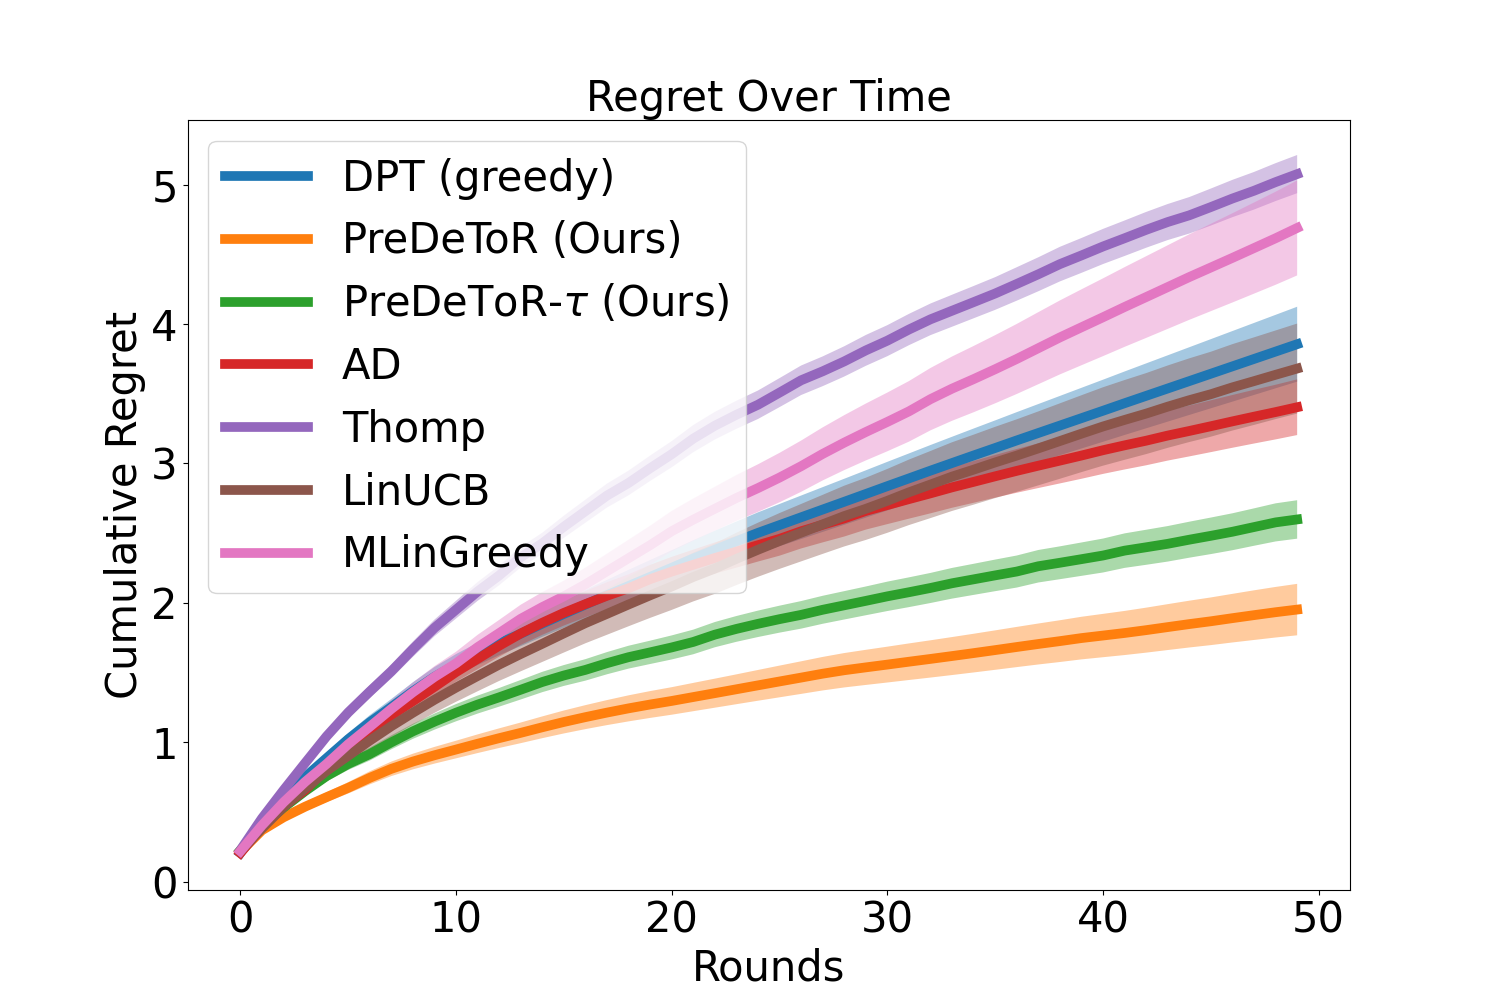
\includegraphics[scale = 0.1]{img/Neurips/non_linear/nlm_lr0.00015_do0_embd32_layer4_head4_envs100001_hists1_samples1_var0.3_cov0.0_H50_d6_lind2_seed1_testcov0.0_hor50.pkl.png} \label{fig:short-horizon-nlm}} &%\\
% %%%%%%%%%%%%%%%%%%%%%%%
% \hspace*{-1.5em}\subfigure[Feature bandit]{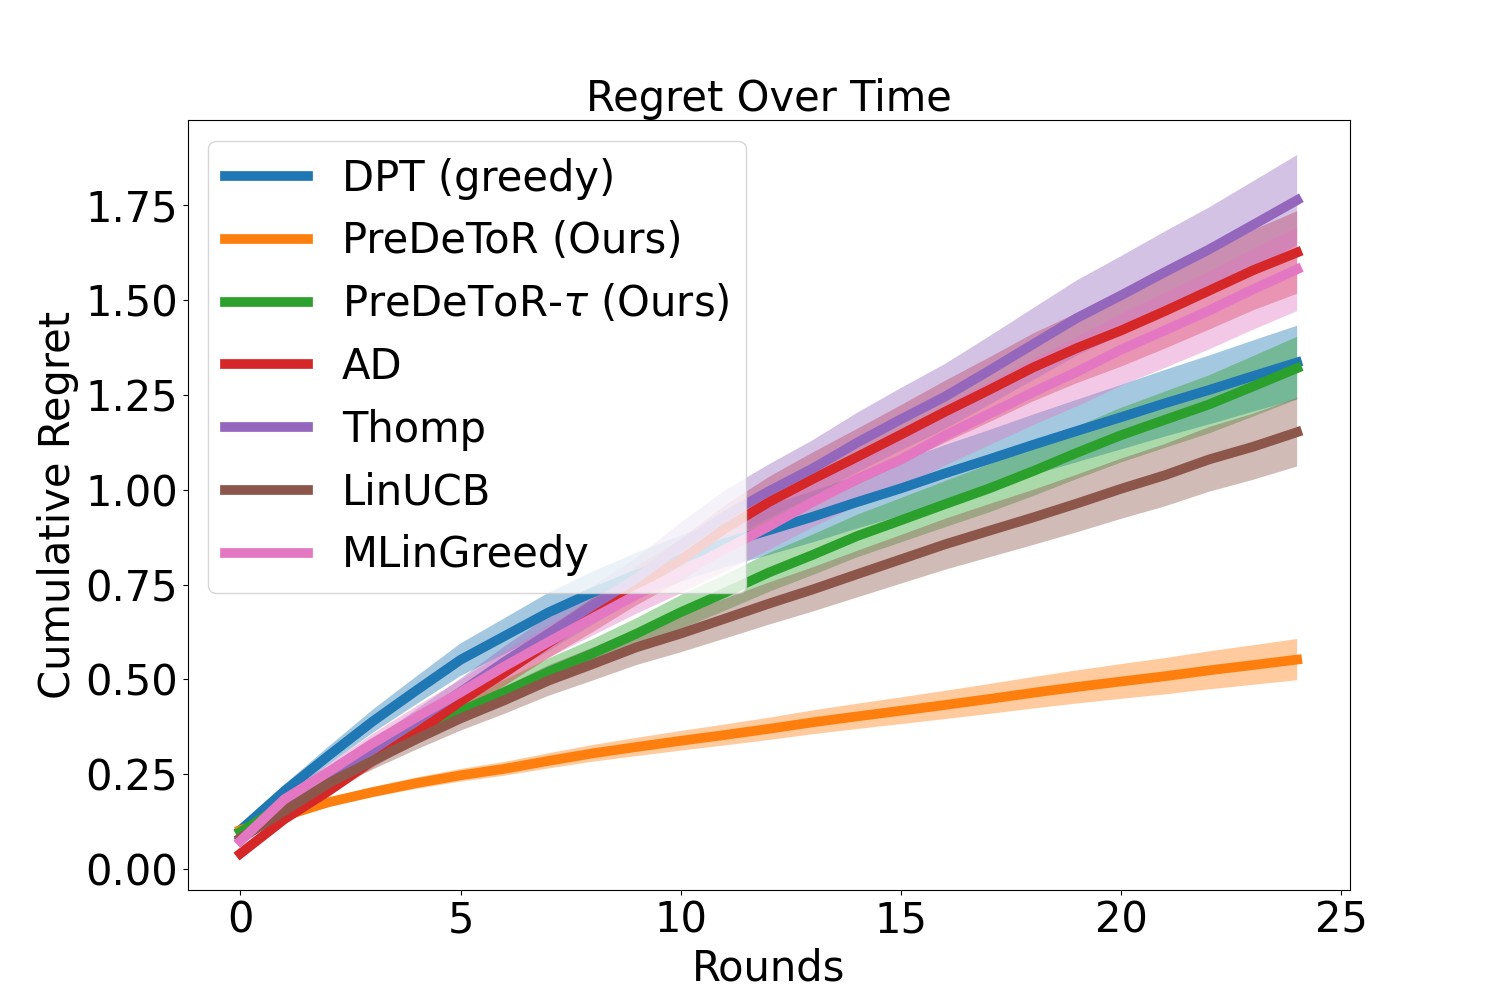
\includegraphics[scale = 0.1]{img/Neurips/non_linear/nlm_wheel_lr0.00015_do0_embd32_layer4_head4_envs101000_hists1_samples1_var0.3_cov0.0_H25_d10_lind2_seed1_testcov0.0_hor25.pkl.png} \label{fig:short-horizon-nlm-feature}}&
% % %%%%%%%%%%
% \hspace*{-1.5em}\subfigure[Movielens]{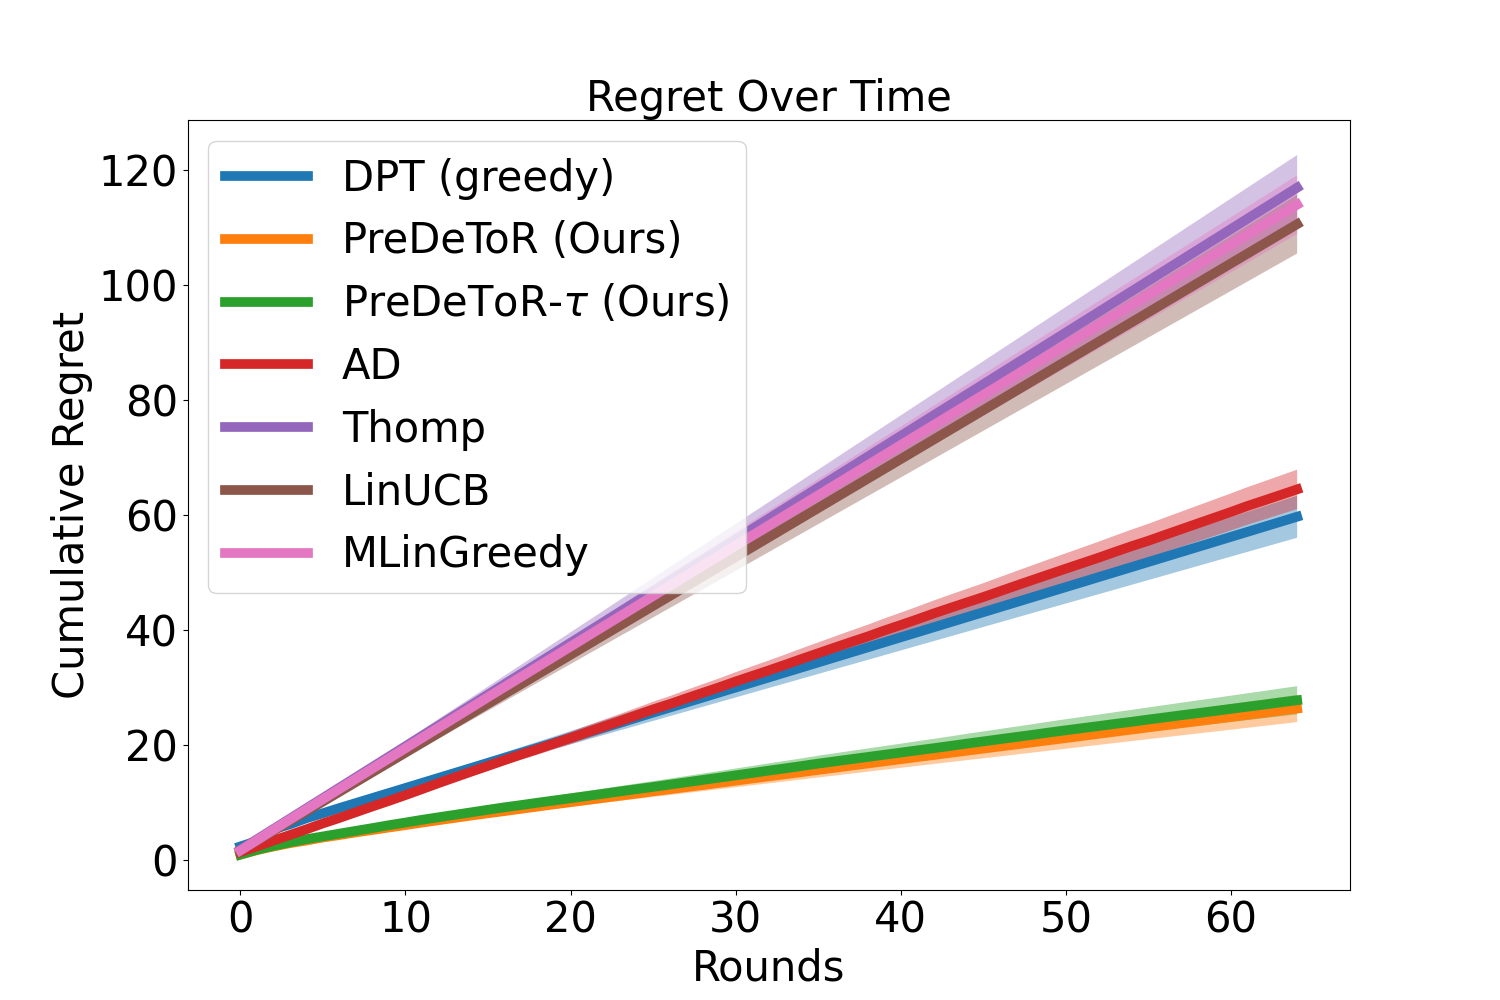
\includegraphics[scale = 0.1]{img/Neurips/non_linear/movielens_lr0.00015_do0_embd32_layer4_head4_envs99800_hists1_samples1_var0.3_cov0.0_H65_d10_lind2_seed1_testcov0.0_hor65.pkl.png} \label{fig:short-horizon-movielens}}&
% % %%%%%%%%%%
% \hspace*{-1.5em}\subfigure[Yelp]{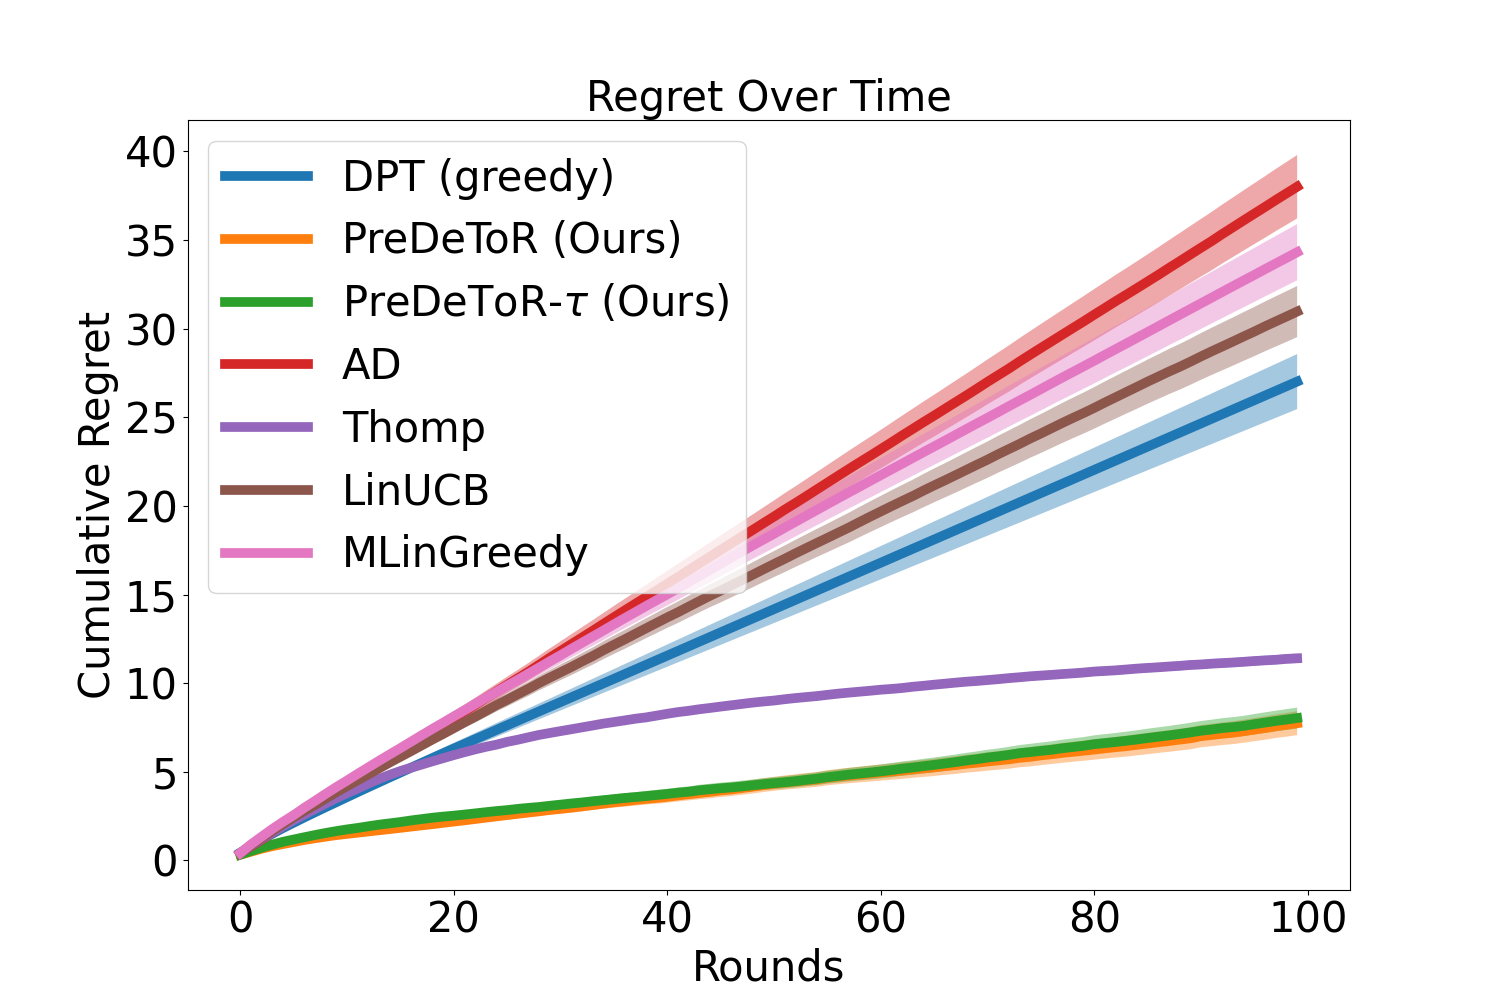
\includegraphics[scale = 0.1]{img/Neurips/non_linear/yelp_lr0.00015_do0_embd32_layer4_head4_envs47757_hists1_samples1_var0.3_cov0.0_H100_d10_lind2_seed1_testcov0.0_hor100.pkl.png} \label{fig:short-horizon-yelp}}
% \end{tabular}
% \vspace*{-1em}
% \caption{Non-linear regime. The horizontal axis is the number of rounds. Confidence bars show one standard error.}
% \label{fig:expt-short-horizon}
% \vspace{-0.7em}
% \end{figure}

\begin{figure}[!hbt]
\centering
\vspace*{-1em}
% Comment out for reference
% \begin{subfigure}[b]{0.25\textwidth}
%     \includegraphics[scale=0.1]{img/Neurips/linear/lin_lr0.00015_do0_embd32_layer4_head4_envs200000_hists1_samples1_var0.3_cov0.0_H25_d10_lind2_seed1_testcov0.0_hor25.pkl.png}
%     \caption{Linear Bandit setting}
%     \label{fig:short-horizon-lin}
% \end{subfigure}%
\begin{subfigure}[b]{0.25\textwidth}
    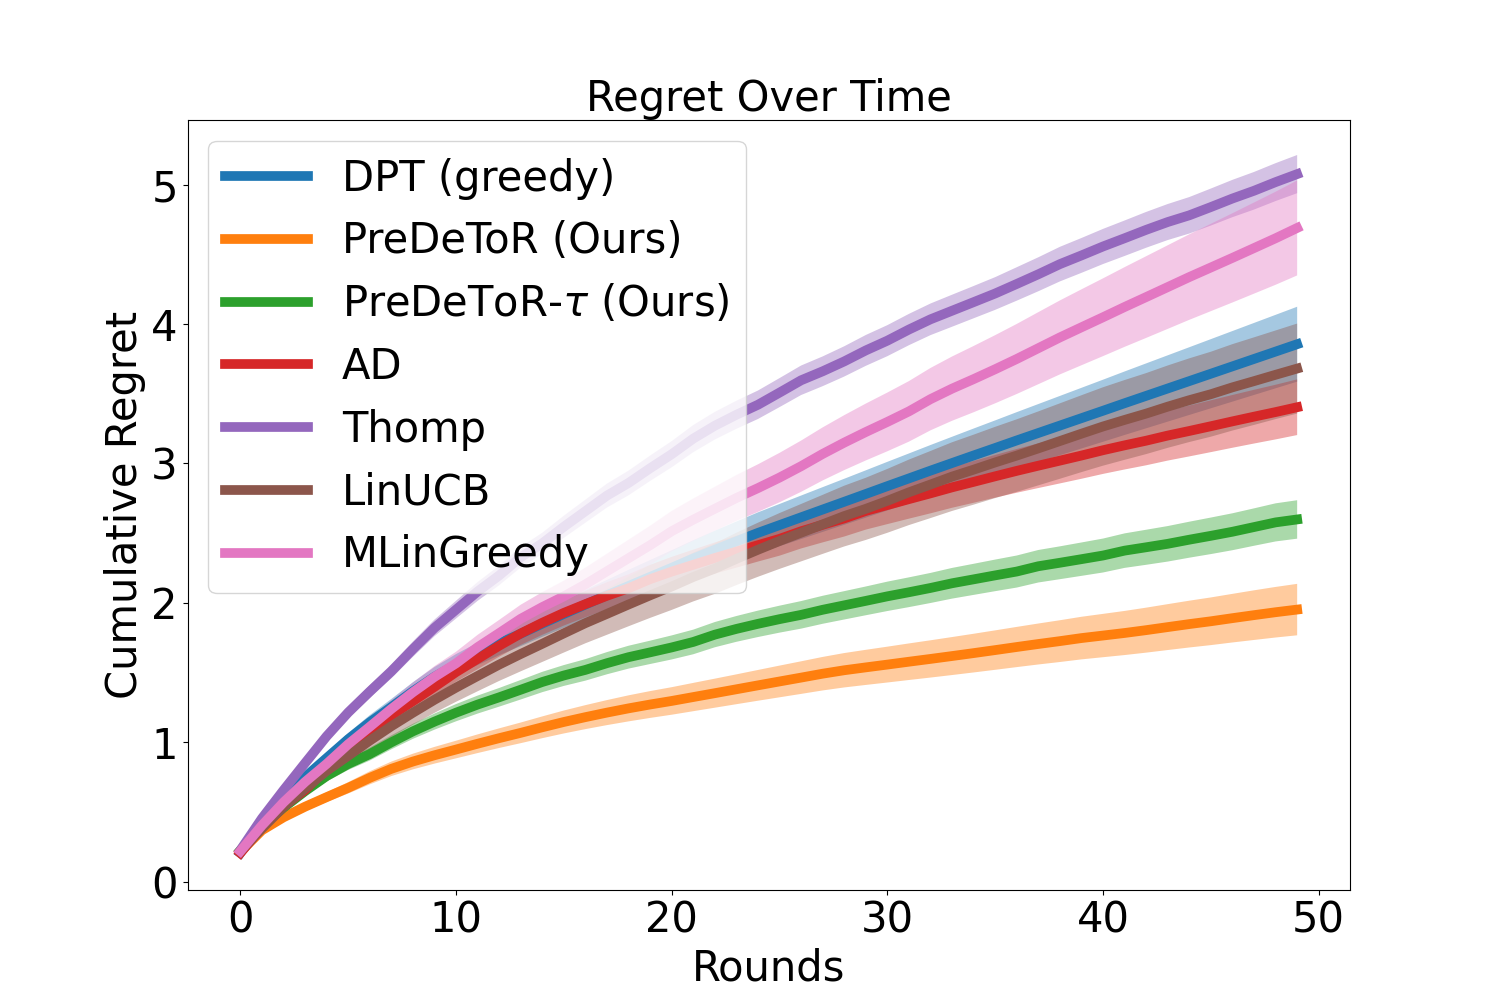
\includegraphics[scale=0.1]{img/Neurips/non_linear/nlm_lr0.00015_do0_embd32_layer4_head4_envs100001_hists1_samples1_var0.3_cov0.0_H50_d6_lind2_seed1_testcov0.0_hor50.pkl.png}
    \caption{Non-linear bandit}
    \label{fig:short-horizon-nlm}
\end{subfigure}%
\begin{subfigure}[b]{0.25\textwidth}
    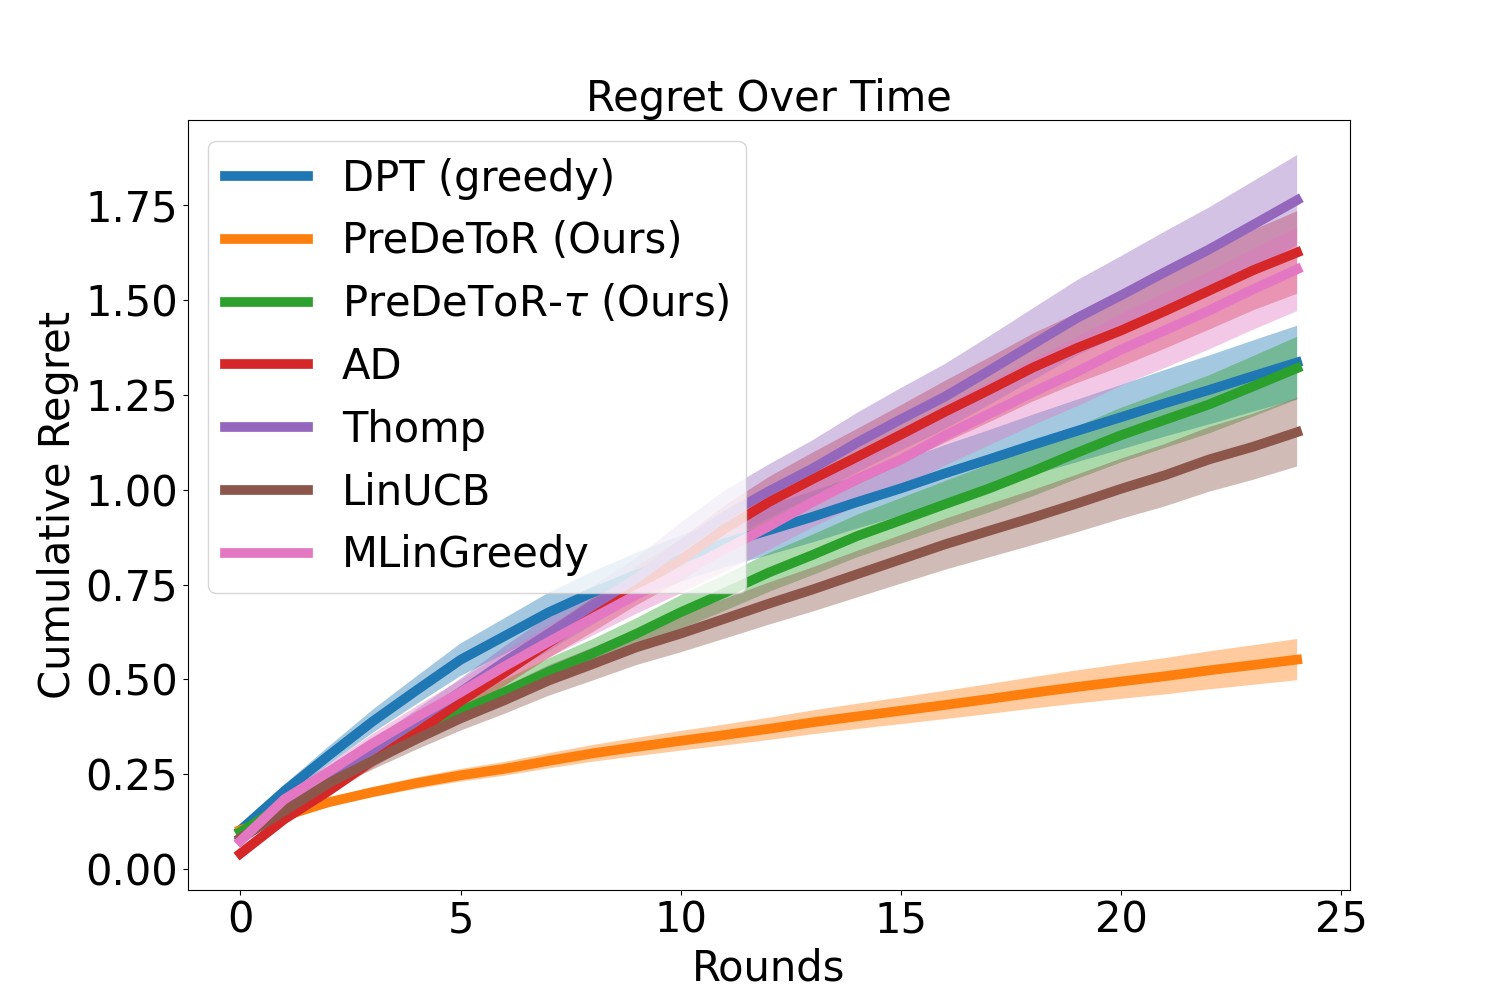
\includegraphics[scale=0.1]{img/Neurips/non_linear/nlm_wheel_lr0.00015_do0_embd32_layer4_head4_envs101000_hists1_samples1_var0.3_cov0.0_H25_d10_lind2_seed1_testcov0.0_hor25.pkl.png}
    \caption{Feature bandit}
    \label{fig:short-horizon-nlm-feature}
\end{subfigure}%
\begin{subfigure}[b]{0.25\textwidth}
    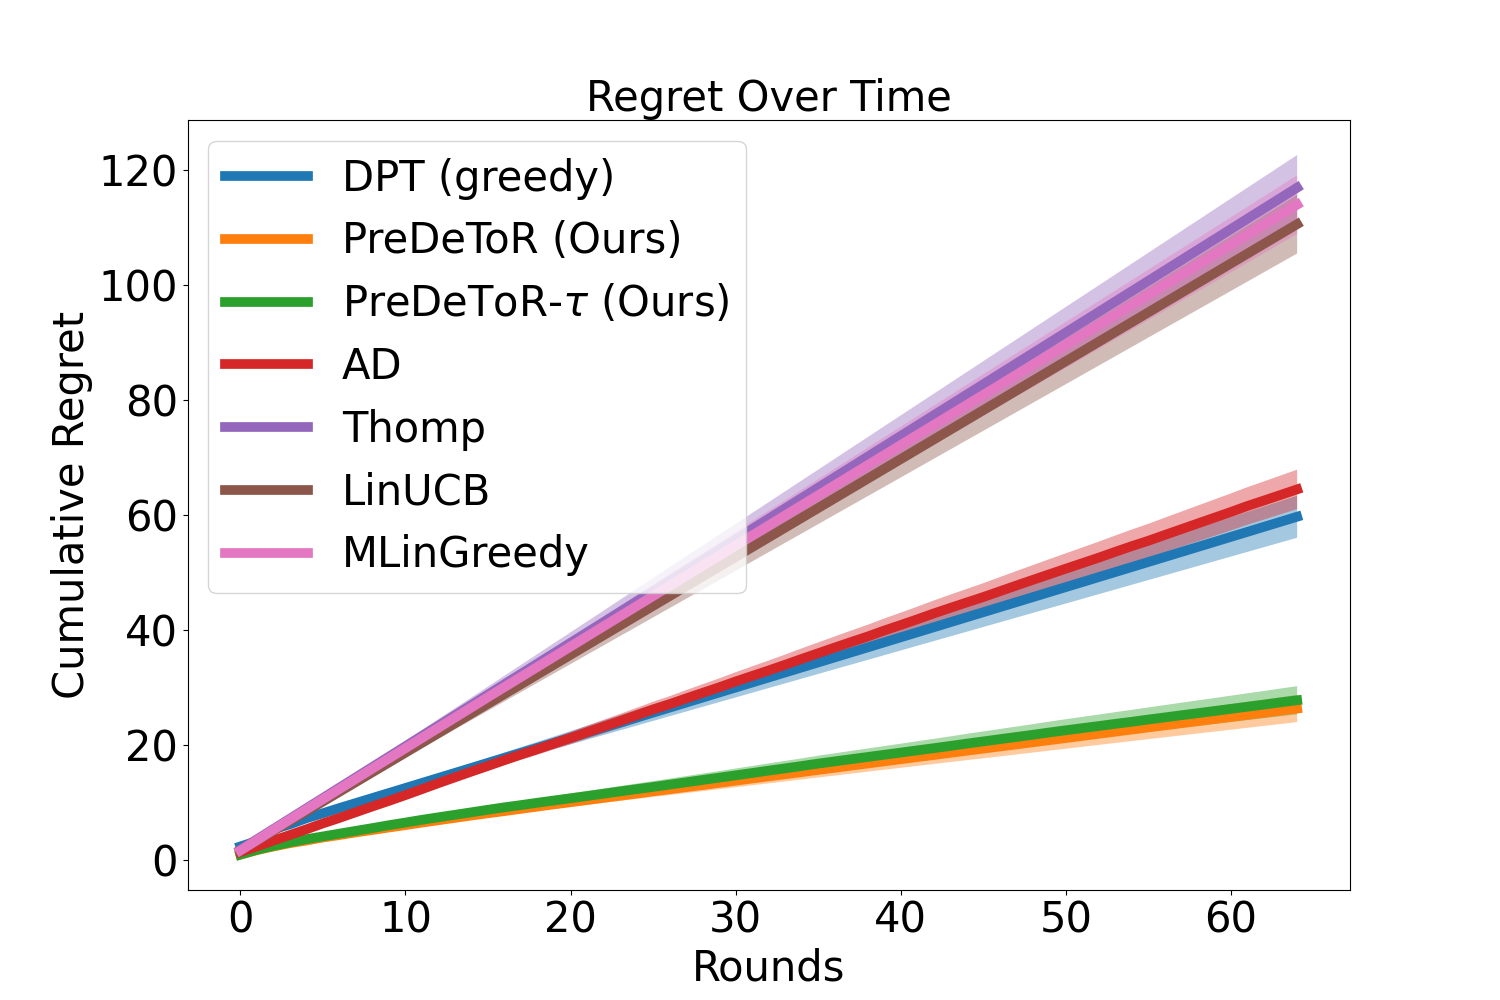
\includegraphics[scale=0.1]{img/Neurips/non_linear/movielens_lr0.00015_do0_embd32_layer4_head4_envs99800_hists1_samples1_var0.3_cov0.0_H65_d10_lind2_seed1_testcov0.0_hor65.pkl.png}
    \caption{Movielens}
    \label{fig:short-horizon-movielens}
\end{subfigure}%
\begin{subfigure}[b]{0.25\textwidth}
    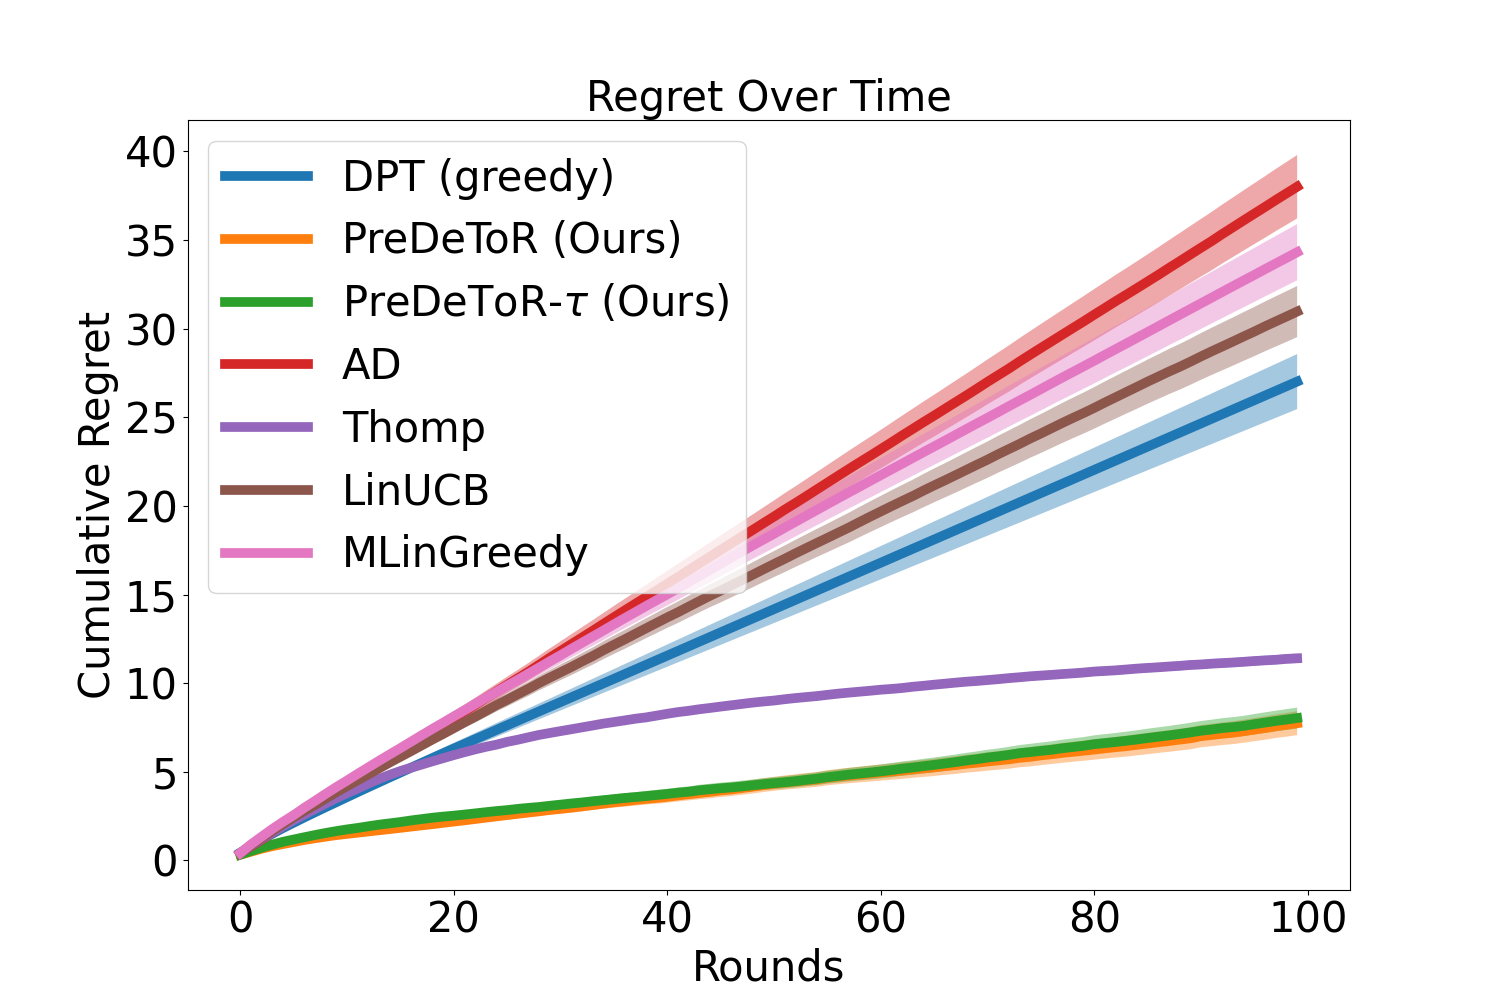
\includegraphics[scale=0.1]{img/Neurips/non_linear/yelp_lr0.00015_do0_embd32_layer4_head4_envs47757_hists1_samples1_var0.3_cov0.0_H100_d10_lind2_seed1_testcov0.0_hor100.pkl.png}
    \caption{Yelp}
    \label{fig:short-horizon-yelp}
\end{subfigure}
\vspace*{-1em}
\caption{Non-linear regime. The horizontal axis is the number of rounds. Confidence bars show one standard error.}
\label{fig:expt-short-horizon}
\vspace{-0.7em}
\end{figure}

